\documentclass[final]{beamer}
\mode<presentation>{\usetheme{I6pd2}}
\usepackage[english]{babel}
\usepackage[latin1]{inputenc}
\usepackage{amsmath,amsthm, amssymb, latexsym}
%\usepackage{times}\usefonttheme{professionalfonts}  % obsolete
\usefonttheme[onlymath]{serif}
\boldmath
\usepackage[orientation=landscape,size=a0,scale=1.4,grid]{beamerposter}
% change list indention level
%\setdefaultleftmargin{3em}{}{}{}{}{}

\usepackage{snapshot} % will write a .dep file with all dependencies, allows for easy bundling

\listfiles

%%%%%%%%%%%%%%%%%%%%%%%%%%%%%%%%%%%%%%%%%%%%%%%%%%%%%%%%%%%%%%%%%%%%%%%%%%%%%%%%%%%%%%
\graphicspath{{figures/}}
 
\title{\huge REU Fish Tracking Project}
%\subtitle{Presentation Subtitle} % (optional)

%% author and in []: shortauthor
\author{Joseph Anderson, Brian Lewis, Colin O'Byrne}
% - Use the \inst{?} command only if the authors have different
%   affiliation.
\institute[University of New Orleans] % (optional, but mostly needed)
{
%  \inst{1}%
 Training and Research in Advanced Computing Knowledge, University of New Orleans, Louisianna
%  \and
%  \inst{2}%
%  Department of Theoretical Philosophy\\
%  University of Elsewhere
}
% - Use the \inst command only if there are several affiliations.
% - Keep it simple, no one is interested in your street address.

\date[12 July 2011]{12 July 2011}
%%%%%%%%%%%%%%%%%%%%%%%%%%%%%%%%%%%%%%%%%%%%%%%%%%%%%%%%%%%%%%%%%%%%%%%%%%%%%%%%%%%%%%
\newlength{\columnheight}
\setlength{\columnheight}{65cm}

%%%%%%%%%%%%%%%%%%%%%%%%%%%%%%%%%%%%%%%%%%%%%%%%%%%%%%%%%%%%%%%%%%%%%%%%%%%%%%%%%%%%%%
\begin{document}
\begin{frame}
  \begin{columns}
    % ---------------------------------------------------------%
    % Set up a column 
    \begin{column}{.33\textwidth}
      \begin{beamercolorbox}[center,wd=\textwidth]{postercolumn}
        \begin{minipage}[T]{.95\textwidth} % tweaks the width, makes a new \textwidth
          \parbox[t][\columnheight]{\textwidth}{ % must be some better way to set the the height, width and textwidth simultaneously
            % Since all columns are the same length, it is all nice and tidy.  You have to get the height empirically
            % ---------------------------------------------------------%
            % fill each column with content            
            \begin{block}{Introduction}
              The goal is to extract and classify fish data from natural underwater video data.  To do this, we use automatic thresholding methods to segment the image and the segmented fish are interpreted by either a system of neural networks or feature extraction algorithms.  We study the performance of different threshold methods and the accuracy of various neural network structures.  WARP methods and Gabor filters are used as classification 
            \end{block}
            \vfill
            \begin{block}{Feature Extraction}
              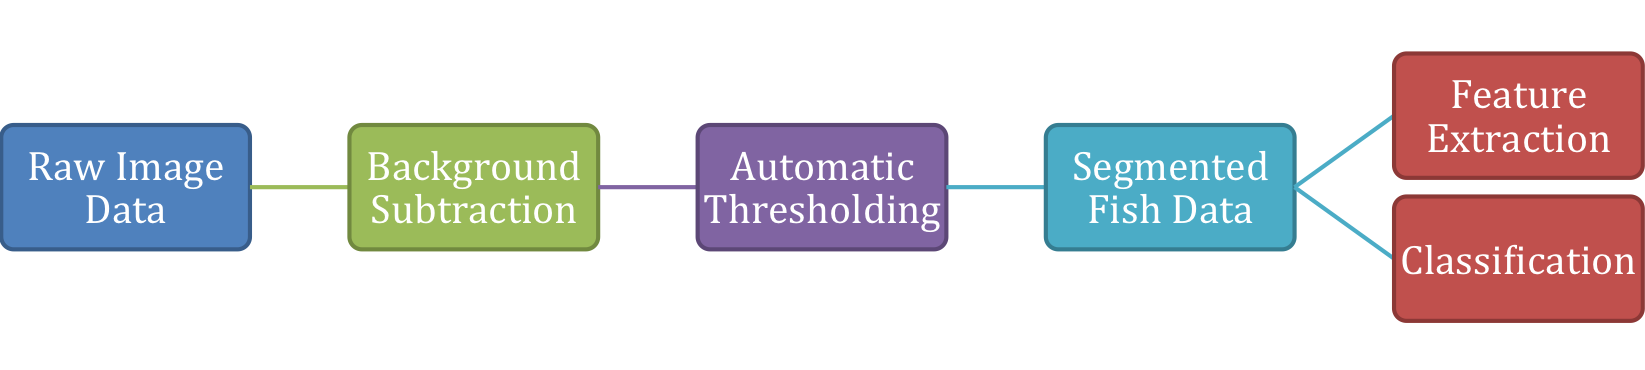
\includegraphics[width=.95\linewidth]{figures/process}
            \end{block}
            \vfill
            \begin{block}{Feature Extraction}
              blah blah blah
            \end{block}
            \vfill
            \begin{block}{Feature Description}
              blah blah blah
            \end{block}
            \vfill
            \begin{block}{Feature Matching}
              blah blah blah
            \end{block}
          }
        \end{minipage}
      \end{beamercolorbox}
    \end{column}
    % ---------------------------------------------------------%
    % end the column

    % ---------------------------------------------------------%
    % Set up a column 
    \begin{column}{.33\textwidth}
      \begin{beamercolorbox}[center,wd=\textwidth]{postercolumn}
        \begin{minipage}[T]{.95\textwidth} % tweaks the width, makes a new \textwidth
          \parbox[t][\columnheight]{\textwidth}{ % must be some better way to set the the height, width and textwidth simultaneously
            % Since all columns are the same length, it is all nice and tidy.  You have to get the height empirically
            % ---------------------------------------------------------%
            % fill each column with content
            
            \begin{block}{Motivation}
              blah blah blah
            \end{block}
            \vfill
            \begin{block}{Methods}
              \begin{itemize}
              \item blah
              \item blah
              \item blah
              \item blah
              \item blah
              \item blah
              \item blah
              \item blah
              \item blah
              \end{itemize}              
            \end{block}
            \vfill
            \begin{block}{Some other thing}
              blah blah blah
            \end{block}
            \vfill
            \begin{block}{Some other thing}
              \begin{itemize}
              \item blah
              \item blah
              \item blah
              \end{itemize}              
            \end{block}
            \vfill
            \begin{block}{Some other thing}
              blah blah blah

              blah blah blah

              blah blah blah

              blah blah blah

              blah blah blah

              blah blah blah

              blah blah blah

              blah blah blah

              blah blah blah
            \end{block}
          }
        \end{minipage}
      \end{beamercolorbox}
    \end{column}
    % ---------------------------------------------------------%
    % end the column

    % ---------------------------------------------------------%
    % Set up a column 
    \begin{column}{.33\textwidth}
      \begin{beamercolorbox}[center,wd=\textwidth]{postercolumn}
        \begin{minipage}[T]{.95\textwidth} % tweaks the width, makes a new \textwidth
          \parbox[t][\columnheight]{\textwidth}{ % must be some better way to set the the height, width and textwidth simultaneously
            % Since all columns are the same length, it is all nice and tidy.  You have to get the height empirically
            % ---------------------------------------------------------%
            % fill each column with content
            
            \begin{block}{Motivation}
              blah blah blah
            \end{block}
            \vfill
            \begin{block}{Some other thing}
              blah blah blah
            \end{block}
            \vfill
            \begin{block}{Some other thing}
              \begin{itemize}
              \item blah
              \item blah
              \item blah
              \end{itemize}              
            \end{block}
            \vfill
            \begin{block}{Some other thing}
              blah blah blah

              blah blah blah

              blah blah blah

              blah blah blah

              blah blah blah

              blah blah blah

              blah blah blah

              blah blah blah

              blah blah blah
            \end{block}
          }
        \end{minipage}
      \end{beamercolorbox}
    \end{column}
    % ---------------------------------------------------------%
    % end the column


  \end{columns}
\end{frame}
\end{document}


%%%%%%%%%%%%%%%%%%%%%%%%%%%%%%%%%%%%%%%%%%%%%%%%%%%%%%%%%%%%%%%%%%%%%%%%%%%%%%%%%%%%%%%%%%%%%%%%%%%%
%%% Local Variables: 
%%% mode: latex
%%% TeX-PDF-mode: t
%%% End:
